\section{Cut-Off}

In Abbildung \ref{fig:plot2} sehen wir den Vergleich der Größenordnungen der eigentlichen Singulärwerte mit den zusätzlichen Singulärwerten.
Nachdem hier ein deutlicher Abfall zu erkennen ist, ist es nicht schwer, die zusätzlichen Werte auszusortieren.

\begin{figure}[H]
  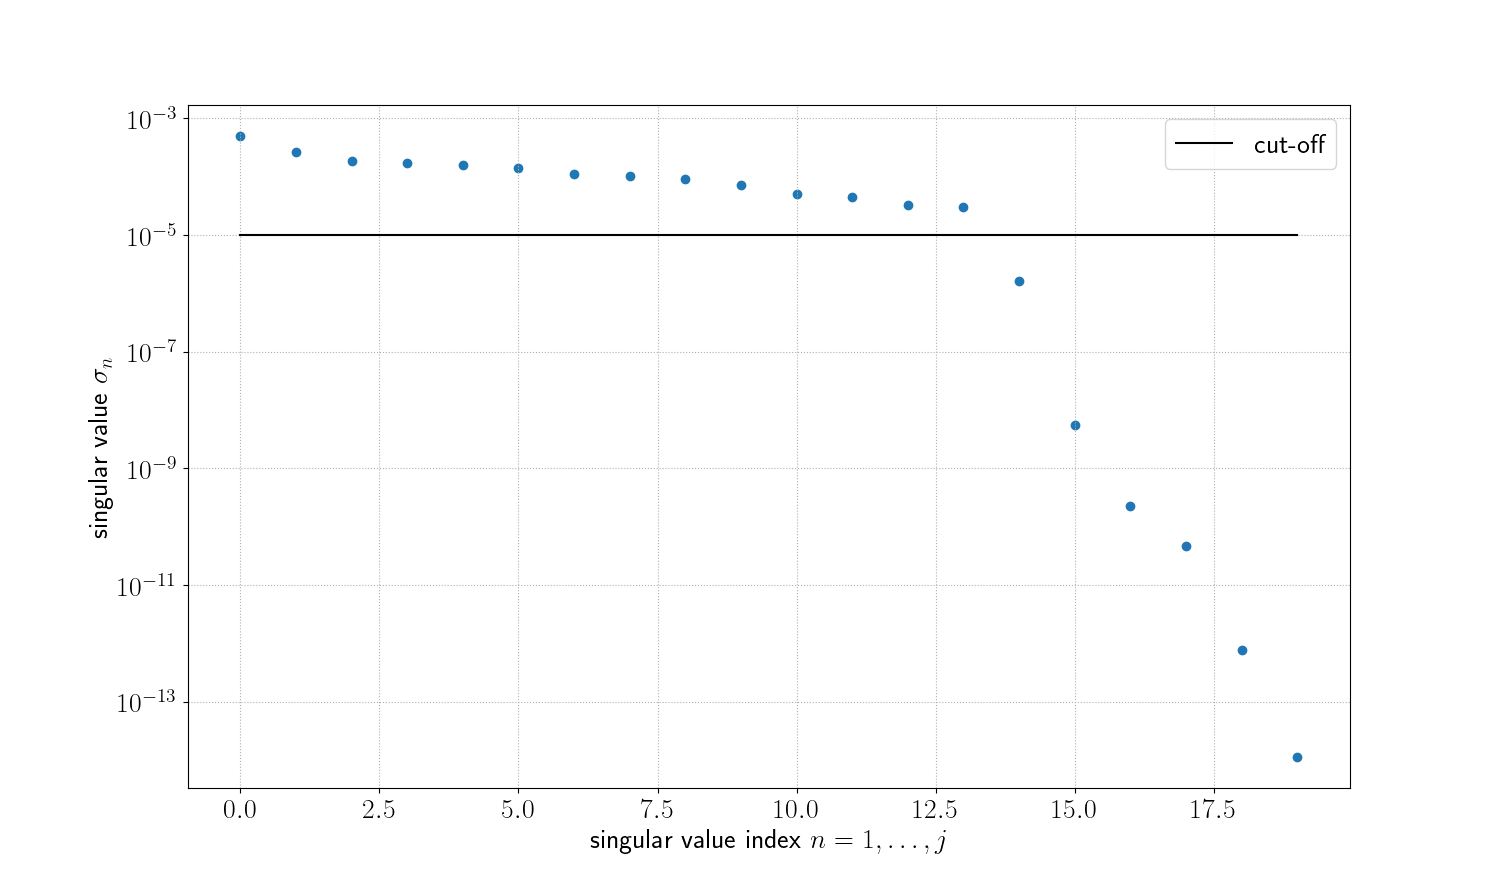
\includegraphics[width = \linewidth]{Plots/singulaerwerte_plot.png}
  \caption{Echte vs. zusätzliche Singulärwerte}
  \label{fig:plot2}
\end{figure}

Eine Heuristik zur Überprüfung der Qualität eines approximierten Eigenwerts $\lambda$ besteht darin, die Konditionszahl der jeweiligen Matrix $A(\lambda)$ zu betrachten.
Da wir gegen eine singuläre Matrix konvergieren sollten, würden wir erwarten, dass die Konditionszahl gegen unendlich geht.
In der Tat ist das Fall und man erkennt in Abbildung \ref{fig:plot3} sogar einen deutlichen Unterschied zwischen den echten und zusätzlichen Eigenwerten.

\begin{figure}[H]
  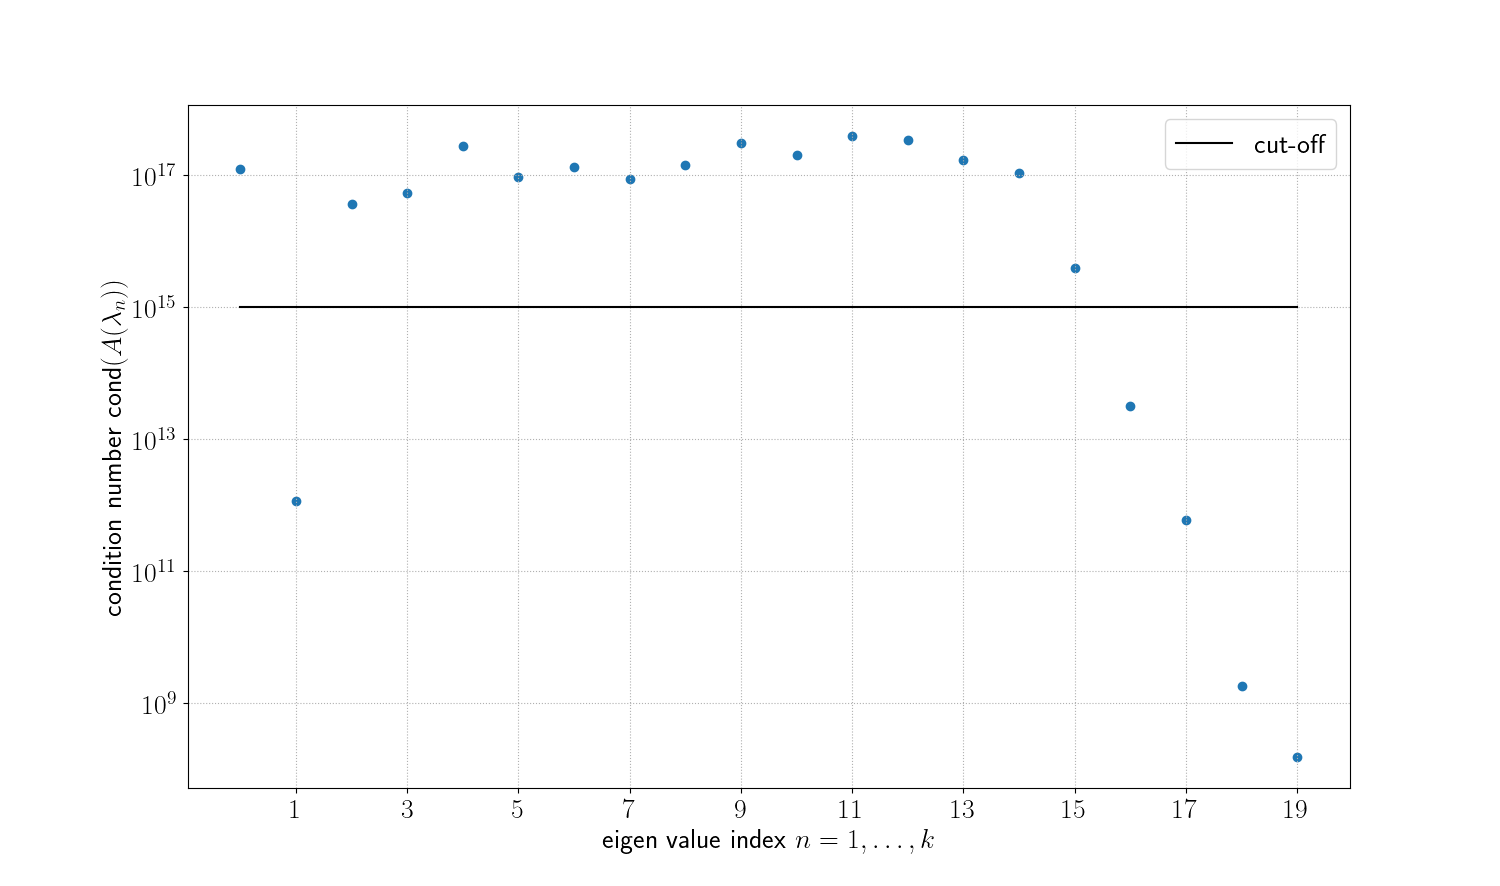
\includegraphics[width = \linewidth]{Plots/conditionnumber.png}
  \caption{Konditionszahlen von $A(\lambda_n)$}
  \label{fig:plot3}
\end{figure}
